\documentclass{article}\usepackage[]{graphicx}\usepackage[]{color}
%% maxwidth is the original width if it is less than linewidth
%% otherwise use linewidth (to make sure the graphics do not exceed the margin)
\makeatletter
\def\maxwidth{ %
  \ifdim\Gin@nat@width>\linewidth
    \linewidth
  \else
    \Gin@nat@width
  \fi
}
\makeatother

\definecolor{fgcolor}{rgb}{0.345, 0.345, 0.345}
\newcommand{\hlnum}[1]{\textcolor[rgb]{0.686,0.059,0.569}{#1}}%
\newcommand{\hlstr}[1]{\textcolor[rgb]{0.192,0.494,0.8}{#1}}%
\newcommand{\hlcom}[1]{\textcolor[rgb]{0.678,0.584,0.686}{\textit{#1}}}%
\newcommand{\hlopt}[1]{\textcolor[rgb]{0,0,0}{#1}}%
\newcommand{\hlstd}[1]{\textcolor[rgb]{0.345,0.345,0.345}{#1}}%
\newcommand{\hlkwa}[1]{\textcolor[rgb]{0.161,0.373,0.58}{\textbf{#1}}}%
\newcommand{\hlkwb}[1]{\textcolor[rgb]{0.69,0.353,0.396}{#1}}%
\newcommand{\hlkwc}[1]{\textcolor[rgb]{0.333,0.667,0.333}{#1}}%
\newcommand{\hlkwd}[1]{\textcolor[rgb]{0.737,0.353,0.396}{\textbf{#1}}}%

\usepackage{framed}
\makeatletter
\newenvironment{kframe}{%
 \def\at@end@of@kframe{}%
 \ifinner\ifhmode%
  \def\at@end@of@kframe{\end{minipage}}%
  \begin{minipage}{\columnwidth}%
 \fi\fi%
 \def\FrameCommand##1{\hskip\@totalleftmargin \hskip-\fboxsep
 \colorbox{shadecolor}{##1}\hskip-\fboxsep
     % There is no \\@totalrightmargin, so:
     \hskip-\linewidth \hskip-\@totalleftmargin \hskip\columnwidth}%
 \MakeFramed {\advance\hsize-\width
   \@totalleftmargin\z@ \linewidth\hsize
   \@setminipage}}%
 {\par\unskip\endMakeFramed%
 \at@end@of@kframe}
\makeatother

\definecolor{shadecolor}{rgb}{.97, .97, .97}
\definecolor{messagecolor}{rgb}{0, 0, 0}
\definecolor{warningcolor}{rgb}{1, 0, 1}
\definecolor{errorcolor}{rgb}{1, 0, 0}
\newenvironment{knitrout}{}{} % an empty environment to be redefined in TeX

\usepackage{alltt}

\usepackage{amsmath, amssymb}
\usepackage{graphicx}
\usepackage{hyperref}
\IfFileExists{upquote.sty}{\usepackage{upquote}}{}
\begin{document}

\title{Pol Sci 630:  Problem Set 12: Heteroskedasticity, Autocorrelation}

\author{Prepared by: Anh Le (\href{mailto:anh.le@duke.edu}{anh.le@duke.edu})}

\date{Due Date: Tue, Nov 17, 2015, 10 AM (Beginning of Class)}

\maketitle

\begin{knitrout}
\definecolor{shadecolor}{rgb}{0.969, 0.969, 0.969}\color{fgcolor}\begin{kframe}
\begin{alltt}
\hlkwd{rm}\hlstd{(}\hlkwc{list} \hlstd{=} \hlkwd{ls}\hlstd{())}
\hlkwd{library}\hlstd{(ggplot2)}
\end{alltt}
\end{kframe}
\end{knitrout}


\section{Heteroskedasticity (8 points)}

One common cause of heteroskedasticity is that our model does not take into account heterogenous effect across sub-populations. For example, we have a model of spending (dependent var) as a function of income (independent var), and the propensity to spend differs across ethnic groups. Formally,

\begin{align}
spending &= \beta_{ethnic} income + \epsilon
\end{align}

where $\beta{ethnic}$ takes a different value for white, black, and asian. If we don't know about this heterogeneity of propensity to spend across ethnic groups, the graph will show heteroskedasticity:

\begin{knitrout}
\definecolor{shadecolor}{rgb}{0.969, 0.969, 0.969}\color{fgcolor}
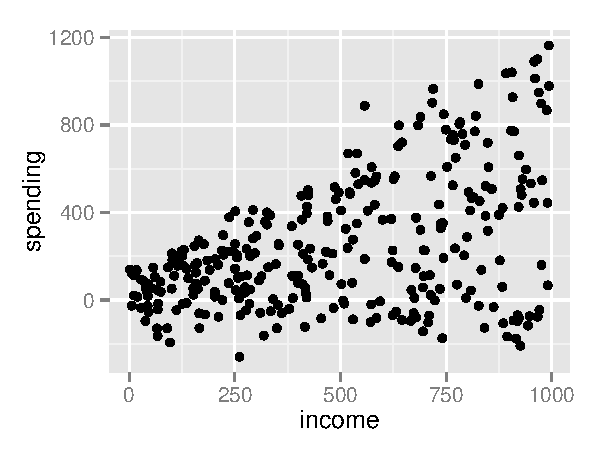
\includegraphics[width=\maxwidth]{figure/unnamed-chunk-2-1} 

\end{knitrout}

Buf if we are smart researcher, we'll realize the underlying cause of the heterogeneity, as shown in the following plot:

\begin{knitrout}
\definecolor{shadecolor}{rgb}{0.969, 0.969, 0.969}\color{fgcolor}
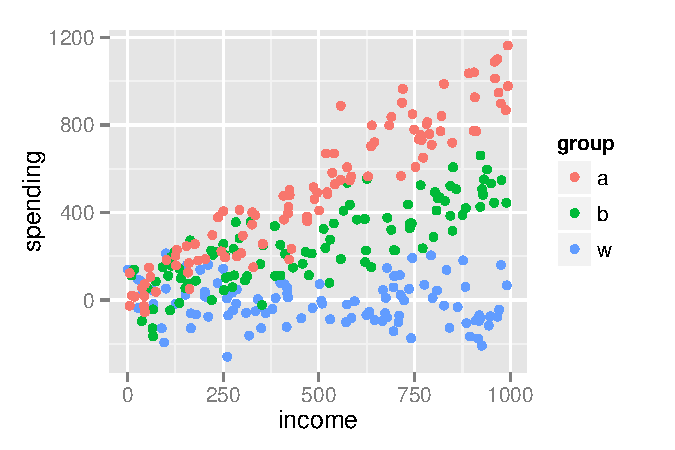
\includegraphics[width=\maxwidth]{figure/unnamed-chunk-3-1} 

\end{knitrout}

The take-home point is that heteroskedasticity could be a signal of underlying model specification, and we should think hard about the cause of heteroskedasticity instead of applying a quick fix.

\subsection{Simulating}

Simulate the spending and income pattern for three ethnic groups as described above. Re-create the two plots above. The numbers don't have to be the same -- just make sure that your data has heteroskedasticity due to underlying heterogenous effect across ethnic groups as described in the example above. Note: Don't look at my code.

\subsection{Diagnostics: Visual}

Using the simulated data above, regress spending on income, plot the residual against the predicted value.

\subsection{Diagonistics: Hypothesis test}

Conduct BP test and White test. Why do the tests reach the same conclusion here, unlike in the lab tutorial?

\subsection{Fixing: robust standard error}

Run hypothesis test without and with robust standard error. What's the conclusion?

\subsection{Fixing: FGLS}

Conduct FGLS. Hint: For stability, log transform $residual^2$ in the auxiliary regression, then exponentiate the predicted value of the auxiliary regression to get the weight.

\subsection{Fixing: Provide a correct model}

Specify a regression model that takes into account heterogenous effect of income on spending across ethnic groups. Show that there's no longer heteroskedasticity.

\section{Multicollinearity (4 points)}

\subsection{Diagnosing with VIF}

Using dataset \verb`Prestige`, run regression of prestiage against income, education, and women. Calculate VIF. Interpret the largest VIF.

\subsection{Dealing with multicollinearity}

If you are concerned that the VIF is causing your SEs to be pretty big. What should you do to address this issue?

\section{Diagnosing autocorrelation (4 points)}

\subsection{Generating autocorrelated data}

Similar to the lab, generate data (i.e. e, X, Y) that follow an AR(2) process, i.e.:

\begin{align}
v(t) &\sim N(0, 1) \\
e(t) &= a_1e(t-1) + a_2 e(t-2) + v(t) \qquad \text{Important: $a_1 + a_2 < 1$} \\
Y(t) &= X(t) + e(t)
\end{align}

\subsection{Diagnostics: Visual}

Plot residual against time and against lagged , up to 4 lags (e.g. residual ~ lag-1 residual, residual ~ lag-2 residual, etc. up to 4 plots) How does the correlation look across the four plots?

\subsection{Diagnostics: Hypothesis testing}

Regress residuals against X and lag1 and lag2 residuals, and then doing an F test for joint significance in the lagged residuals.

\end{document}
